\documentclass[twocolumn, 9pt]{article}

%encoding
\usepackage[utf8]{inputenc}

%set up margins
\usepackage[top=0.88in, bottom=1.18in, left=0.9in, right=0.9in]{geometry}
\setlength{\columnsep}{0.2in}

%set main font to times new roman
\usepackage{times}

%try to balance last page
\usepackage{flushend}

%set up section title style: 2 empty lines between sections
\makeatletter
\renewcommand\section{\@startsection {section}{1}{\z@}%
                                   {-2\baselineskip}%
                                   {.14in}%
                                   {\hspace{-1em}\large\textbf}}

\makeatother
\makeatletter
\renewcommand\subsection{\@startsection {section}{1}{\z@}%
                                   {-2\baselineskip}%
                                   {0.08in}%
                                   {\hspace{-1em}\textbf}}
\makeatother

%packages for tikz graphs 
\usepackage{pgf}
\usepackage{tikz}
\usepackage{textcomp}
\usetikzlibrary{shapes,arrows,positioning}
\usepackage{varwidth}
\usepackage{amsthm}
\usepackage{amsmath}
\usepackage{amssymb}
\usepackage{graphicx} %draw images
\usepackage{color}    %colorize text
\usepackage{placeins} %float barrier
\usepackage{url}
\usepackage[square, numbers, comma, sort&compress]{natbib}
\usepackage[hidelinks]{hyperref}
\hypersetup{breaklinks=true}
\urlstyle{same}
\Urlmuskip=0mu plus 1mu

% Defining string as labels of certain blocks.
\newcommand{\cm}[1]{{\color{red}#1}}

\title{Visualisation and Analysis of Geographic Information: Finding Representative Points of Interest}


%
\author{
\begin{tabular}{c c}
João Valença 			   & Luís Paquete 				\\
CISUC/DEI/University of Coimbra				   & CISUC/DEI/University of Coimbra					\\
Coimbra, Portugal		   & Coimbra, Portugal 			\\
valenca@student.dei.uc.pt  & paquete@dei.uc.pt 			\\
						   & 							\\
Pedro Reino  			   & Carlos Caçador				\\
Smartgeo Solutions  	   & Smartgeo Solutions			\\
Lisboa, Portugal    	   & Lisboa, Portugal			\\
pedro.reino@smartgeo.pt    & carlos.cacador@smartgeo.pt \\
\end{tabular}
}

\date{}

\begin{document}

\twocolumn[
  \begin{@twocolumnfalse}
    \maketitle
	\begin{abstract}
		This project aims to develop a GIS application operating through a Web platform in order to allow for a low cost and simplified integration, management and manipulation of georeferenced information.
		In particular, the goal is to develop a way to efficiently extract a subset of a collection of geographic points of interest whilst keeping the representativeness of the whole set.
		This problem of finding such representation is recast as a discrete optimisation problem. The approaches covered in this work include exact algorithms for finding minimum coverage subsets, as well as heuristic approaches for finding good approximations in real time.
		
\smallskip

\emph{Keywords:} Geographic Clustering, k-Center, Coverage, Branch-and-Bound, Delaunay Triangulations\\
	\end{abstract}
  \end{@twocolumnfalse}
]

\section{Objective}

One obstacle when representing large amounts of geographic data is that the number of points to display can be overwhelming for a human, as well as computationally intensive to render for a machine. As such, there is a need to develop and implement a viable way to reliably calculate and display a subset of geographic points, whilst keeping a degree of representativeness of the larger set.

The purpose of this project is to develop a real-time algorithmic framework that can analyse geographic data provided by a geographic information system infrastructure. More precisely, the developed algorithm has to be able to aggregate and select geographic points according to a given a set of criteria in real time. The chosen subset should keep a measure of representativeness of the larger set.

Figure \ref{fig:figure1} shows a representative subset of the set of cities, towns and villages in Sweden. The points were taken from a dataset available in \cite{dataset}.

\begin{figure}[h]	
	\centering
	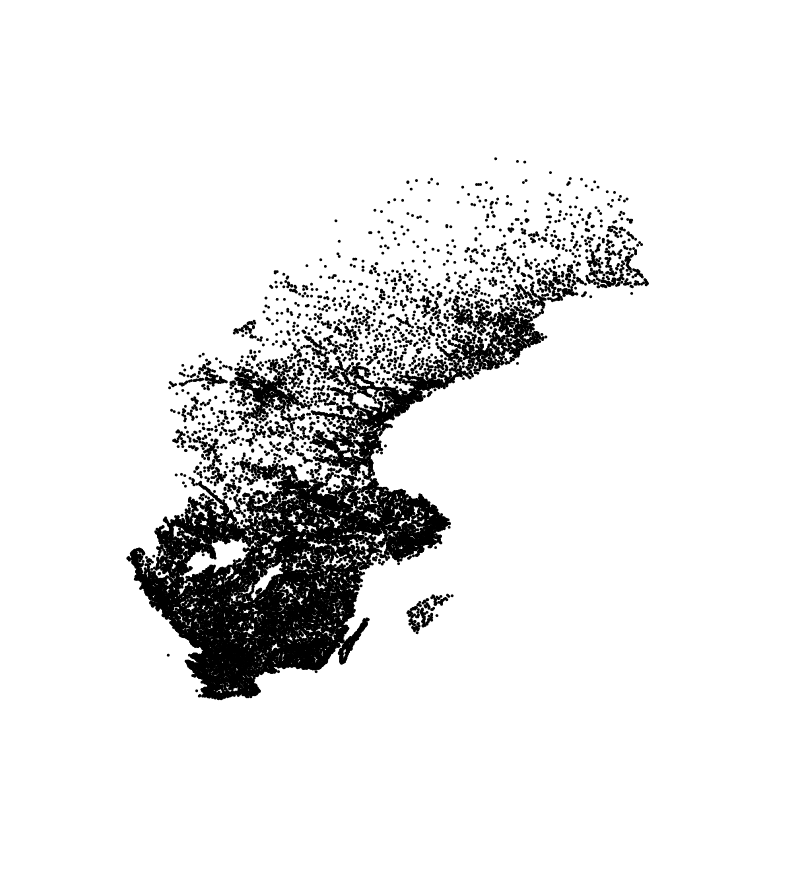
\includegraphics[width=.24\textwidth]{swe1.png}\hfill
	%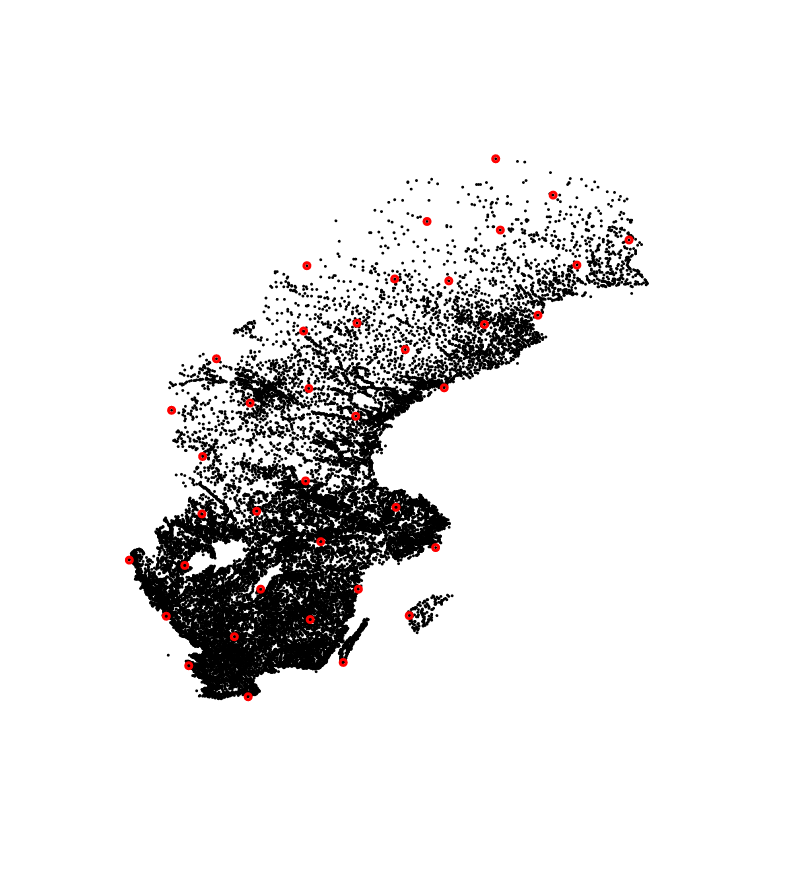
\includegraphics[width=.2\textwidth]{swe2.png}\hfill
	
\includegraphics[width=.24\textwidth]{swe3.png}
	
	\caption{The Sweden dataset (left) and a representative subset (right)}
	\label{fig:figure1}
\end{figure}

\section{Problem Definition}

Representativeness consists of finding a subset of points in a larger set that meets some representation quality. The subset chosen should be able to keep some properties of the original set, such as density, or distribution.

In this work, representativeness is understood as finding the subset that minimises the maximum distance between the the not chosen points, and their closest counterparts within the chosen set. This notion of representativeness is known in discrete optimisation as \emph{coverage}. The problem can be approached by finding the subset of cardinality $k$ that minimises the value of coverage, known as the \emph{k-center} problem \cite{complex}. Another approach is to establish an arbitrary minimum distance and minimise the number of points needed to cover all the remaining points within that distance. This approach can be recast as a set cover problem.

In order to address these problems, algorithms were developed and implemented. Optimal approaches to the problems include integer linear programming, as well as branch-and-bound algorithms. However, the inherent overhead in these algorithms makes them unsuitable for use in real-time applications. For achieving an acceptable approximation to the optimal solution within a reasonable time frame of what is expected in a real-time web application, heuristic methods need to be used.

\section{Architecture}

The application displays a rectangular window, showing a cut of a geographical region containing a small set of points that is representative of all the points of interest within that region. The algorithm chosen must be able to choose a representative set of points within the window quickly, as well as be able to recompute a new set points for a new window, resulting from panning or zooming the display window over the region.

The algorithms tested include exact algorithms for finding the minimum coverage subset for a given cardinality. These are comprised of two branch-and-bound algorithms: a naïve incremental approach and a geometric incremental approach that makes use of the properties of Delaunay triangulations in order to speed up point location queries via the Greedy Routing algorithm \cite{greedy}.
An exact integer linear programming approach is benchmarked as well. This project also includes a few heuristic approaches and approximation algorithm techniques to solve the representation problem more efficiently.

The algorithm serves as the middleware responsible for filtering the response of a GIS server to a Web Feature Service, or WFS request. Finally, a web application receives the response filtered by the algorithm and interacts with a human user. 

The candidate algorithms were tested and benchmarked using data from the Open Street Map project. The project features large quantities of open source geographic data, as well as a versatile API for fetching data.

\section{Results}
The first approach solves the representativeness problem by finding the minimum the coverage subset with a fixed cardinality. The solutions include Branch-and-Bound algorithms, as well as Integer Linear Programming. The performance of these algorithms is too slow even for a small number of points, and takes minutes to solve very small instances of the problem, deeming these algorithms unusable in the context of a web application.

The second approach, i.e.\ minimising the number of points chosen given a fixed minimum distance, was solved using a greedy approximation algorithm to the set cover problem. This algorithm guarantees an approximation with at most $\log_2{N}$ points more than the optimal solution \cite{approx}. This algorithm yielded much faster times, whilst keeping an acceptable quality for the resulting sets. Figures \ref{fig:figure2} and \ref{fig:figure3} plot some results obtained by running the algorithm on a square region with uniformly distributed points. The program was written in $C++$ and compiled using $gcc 4.9.2$ on an Arch Linux Operating System (3.19.2-1-ARCH). The CPU used was an Intel i7 Dual-Core with 2Ghz, and 8Gb of 1600MHz memory.

Figure \ref{fig:figure2} shows the CPU-time in seconds taken by the algorithm with respect to the number of points. A minimum distance was fixed (as a percentage of the region size) for the different runs. For each run, the number of points was varied to plot the CPU time as a function of N.

Figure \ref{fig:figure3} shows the number of points $K$ that the algorithm returned for the representative set with respect to the minimum distance. Each run has a different value for $N$. The minimum distance is varied between 10\% to 45\% of the dimension of the side of the square region.  Smaller values of $K$ represent better solutions.

\begin{figure}[h]	
	\centering
	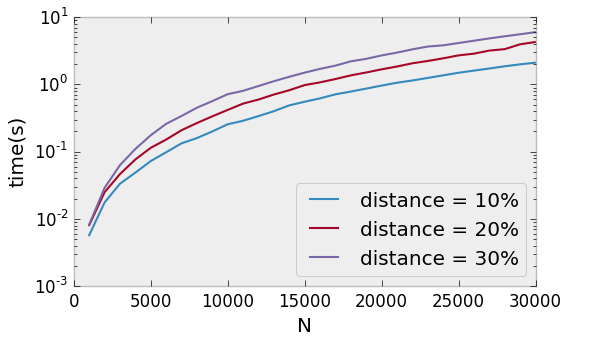
\includegraphics[width=.49\textwidth]{res1.png}
	\caption{CPU time for various values of N}
	\label{fig:figure2}
	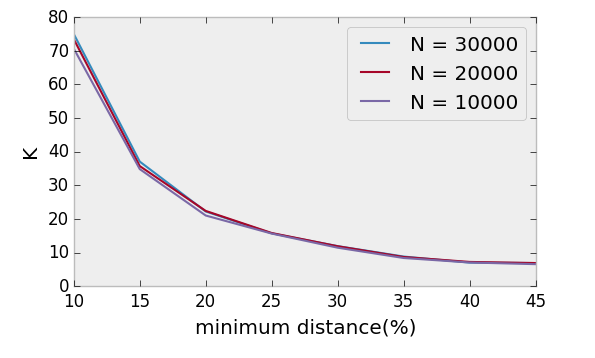
\includegraphics[width=.49\textwidth]{res2.png}
	\caption{Number of points in the covering set with respect to the minimum distance.}
	\label{fig:figure3}
\end{figure}

These results show that the algorithm can be used in the context of a web application. They may still be improved by implementing a more efficient range query search algorithm used in the pre-processing stage of the approximation algorithm. Approaches such as heuristics and other approximation algorithms may also yield better results.

%\begin{table}[h]
%	\begin{center}
%		\begin{tabular}{|c|c|}
%			\hline
%			CPU & Intel i7 Dual-Core, 2GHz\\\hline
%			Memory & 8 GB, 1600 MHz \\\hline
%			Operating System  & Arch Linux 3.19 x86\_64\\\hline
%			Language & \emph{C++} \\\hline
%			Compiler & \emph{gcc 4.9.2} \\\hline
%		\end{tabular}
%		\caption{Machine specifications}
%	\end{center}
%	\label{tab:specs}
%\end{table}

%\FloatBarrier

%\lhead{\emph{References}} % Change the page header to say "Bibliography"

%\bibliographystyle{abbrvnat} % Use the "unsrtnat" BibTeX style for formatting the Bibliography

%\bibliography{Bibliography} % The references (bibliography) information are stored in the file named "Bibliography.bib"
\section*{Acknowledgements}
This work is being developed in the context of the R\&D project QREN unit in co-promotion no.34164 - Smartgeo Portal ”Geographic Information Management System”. The project is co-financed by QREN and Innovation Agency within the scope of the technological development and research incentive system, by the Operational Program for Competitiveness and Internationalizations (Compete).

\bibliographystyle{abbrvnat}
\bibliography{Bibliography}

%\section*{Acknowledgements}
%This work is being developed within the work plan of a research grant for undergraduates, in the context of the R\&D project QREN unit in co-promotion no.34164 - Smartgeo Portal "Geographic Information Management System". The project is co-financed by QREN and Innovation Agency within the scope of the technological development and research incentive system, by the Operational Program for Competitiveness and Internationalization (Compete).
%\bibliography{refs}
\quad
\end{document}